\section{Rigid Body Simulation}
The goal of this project was to develop a game which is based on a real time physics simulation for fluid-structure interaction. The main task of the rigid body group was hence the collision detection and collision handling for the different objects as well as developing the interface to the fluid group, which gives us the necessary two-way-interaction of the fluid and the bodies. 

While the collision between simple shapes like circles and rectangles is manageable, it becomes more complex for polygons. Therefore, whereas the fluid group implemented their own LBM solver, we decided to adapt the real-time physics library \emph{Bullet} \cite{Bullet} for the rigid body handling. By doing this, we did not have to invent the wheel anew. Furthermore, Bullet gives a lot of possibilities for extensions to the program-- offering a variety of different complex shapes for example. Hence, the first approach was to implement Bullet using simple shapes, such as circles and rectangles and then move on to more complex polygons.

\subsection{Bullet}
As a prerequisite, our first task in this project was to get Bullet running on multiple layers-- i.e. understanding the library as well as using it in our project. This task, as simple as it might seem at first sight, already included some pitfalls, which we hope to diminish for the next group with the help of this report. 
\subsubsection{Building}
To build Bullet, one needs \emph{cmake} \cite{CMake}. After having downloaded the project repository \verb+fa+, one can follow the instructions below to build Bullet:
\begin{enumerate}
\item Extract the \verb+fa/sources-for-rigidbody/bullet3-2.83.6.tar.gz+
\item run \verb+cmake .+ in the top directory.
\item run \verb+make -j4+ (\verb+-j4+ chooses 4 threads for compilation) in the top directory.
\item run \verb+sudo make install+ in the \verb+src+ directory.
\end{enumerate}
Afterwards, one has to link to the library in the compilation (usually \verb+/usr/local/include/bullet+ and \verb+-L/usr/local/lib+)
\subsubsection{Functionality we used}
We had three basic classes from Bullet which we used. The first was \verb+btDiscreteDynamicsWorld+, see \autoref{fig: btDDWgraph}. As the class name already states, \verb+btDiscreteDynamicsWorld+ can be seen as the world where the rigid body simulation takes place. It contains all the rigid bodies and all important world parameters, like gravity and size of a timestep for example. By calling \verb+stepSimulation()+ on the world, Bullet performs one simulation step on all the rigid bodies in the world.

\begin{figure}
\centering
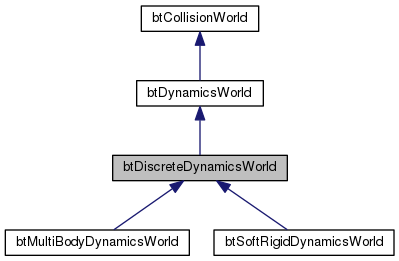
\includegraphics[scale=0.5]{img/RigidBodies/btDiscreteDynamicsWorldGraph.png}
\caption{Inheritance diagram of \texttt{btDiscreteDynamicsWorld}}
\label{fig: btDDWgraph}
\end{figure}

With that, we directly come to Bullet's rigid body class: \verb+btRigidBody+, see \autoref{fig: btRBgraph}. The library offers three kinds of rigid bodies types:
\begin{enumerate}
\item \textbf{Dynamic rigid bodies} with positive mass. Motion is controlled by rigid body dynamics.
\item \textbf{Fixed objects} with zero mass. They are not moving.
\item \textbf{Kinematic objects}, which are objects without mass, but the user can move them.
\end{enumerate}
We used objects of type 1. and 2., which we controlled by assigning them the corresponding mass. Hence, we could build dynamic (floating obstacles) and static objects (walls, boundaries) in our simulation. Furthermore, the \texttt{btRigidBody} class offers methods to access the properties of the objects such as 
\begin{itemize}
\item \texttt{getTotalForce():} Returning the force applied on the object
\item \texttt{getLinearVelocity():} Returning the linear velocity
\item \texttt{getCenterOfMass():} Returning the current center of mass
\end{itemize}
to name a few. 

\begin{figure}
\centering
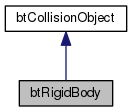
\includegraphics[scale=0.5]{img/RigidBodies/btRigidBodyGraph.png}
\caption{Inheritance diagram of \texttt{btRigidBody}}
\label{fig: btRBgraph}
\end{figure}


Finally, Bullet also offers the possibility to assign a shape to a \texttt{btRigidBody} object. Here, a shape object can be rather seen as a pattern than an actual object, since multiple rigid bodies can share the same shape object. The class in Bullet is called \texttt{btCollisionShape}. See \autoref{fig: btCSgraph} in the appendix, for an inheritance diagram which shows the amount of different shapes this family of classes provides. From convex shapes over concave shapes to compound shapes which one can freely design. The two shapes that we use are \texttt{btCylinderShape} and \texttt{btBoxShape}, see \autoref{fig: btCylSgraph} and \autoref{fig: btBoxSgraph}. By assigning a height of 1 to the cylinder we receive a circle shape; the box shape is used for rectangles and squares. The idea is to later move on to more complex polygons, of course.
\begin{figure}[ht]
\centering
\begin{minipage}{.45\linewidth}
\centering
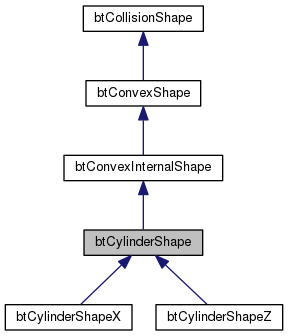
\includegraphics[scale=0.5]{img/RigidBodies/btCylinderShapeGraph.png}
\caption{Inheritance diagram of \texttt{btCylinderShape}}
\label{fig: btCylSgraph}
\end{minipage}
\hspace{.05\linewidth}
\begin{minipage}{.45\linewidth}
\centering
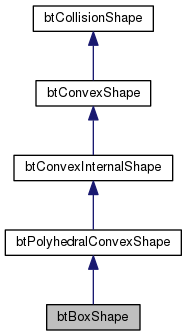
\includegraphics[scale=0.5]{img/RigidBodies/btBoxShapeGraph.png}
\caption{Inheritance diagram of \texttt{btBoxShapeGraph}}
\label{fig: btBoxSgraph}
\end{minipage}
\end{figure}

\subsubsection{Implementation}
In this section we take a look at our actual implementation. For that, the general structure is depicted with the help of an UML diagram, see \autoref{fig: RBUMLgraph}. Although the diagram shows a few of the most important methods, it focusses more on the connection between the classes and the general structure. In the following, we want to give a simple introduction to the individual classes. All of them are also documented with the help of \emph{Doxygen} \cite{Doxygen}. Hence, to get more detailed information about the properties, members and methods of each class, create the Doxygen documentation by calling \texttt{doxygen Doxyfile} in the top most folder of the source code. The main page of the documentation can then be found in \texttt{/html/index.html}.
\begin{figure}[ht]
\centering
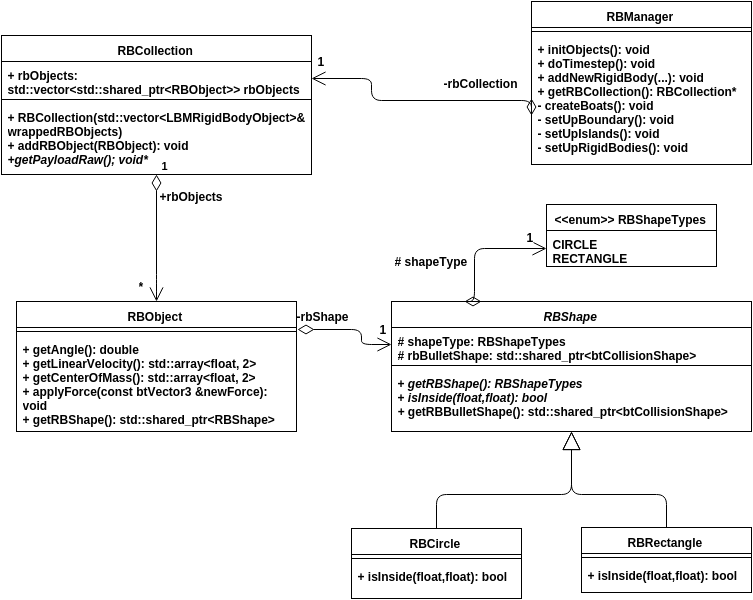
\includegraphics[scale=0.42]{img/RigidBodies/RigidBodyUML.png}
\caption{UML diagram of rigid body classes}
\label{fig: RBUMLgraph}
\end{figure}

\subsubsection*{RBObject and RBShape}
To wrap Bullet, we developed our own classes which we named \texttt{RBObject} and \texttt{RBShape}; they wrap \texttt{btRigidBody} and \texttt{btCollisionShape} respectively. The two specific shapes we implemented by now are \texttt{RBCircle} and \texttt{RBRectangle}, see \autoref{fig: RBShape} for the specific inheritance diagram. \todointern{Benni}{should this be moved to the respective interfaces?} 
\texttt{RBObject} on the other hand includes all the methods from Bullet which we need to transfer information for the LBM simulation and the visualization, like \texttt{getLinearVelocity()} and \texttt{getCenterOfMass()} as mentioned above. 
\begin{figure}[ht]
\centering
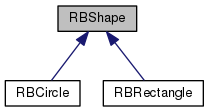
\includegraphics[scale=0.5]{img/RigidBodies/RBShapeGraph.png}
\caption{Inheritance diagram of \texttt{RBShape}}
\label{fig: RBShape}
\end{figure}

\subsubsection*{RBCollection}
<<<<<<< HEAD
\texttt{RBCollection} is a container class for all generated \texttt{RBObjects}. is also responsible for the communication to LBM and visualization, since it is a derived class from \texttt{CPipelinePacket}. With methods like \texttt{getLBMOBjectWrapperBegin()} or \texttt{getPayloadRaw()} it gives access to different pieces of information transferred between the stages. 

\subsubsection*{RBManager}
\label{sec: rbManager}
The class \texttt{RBManager} has a \texttt{btDiscreteDynamicWorld} as member, control over the \texttt{RBCollection} and is hence responsible for the simulation. By calling the class method \texttt{doTimeStep()} one implicitly calls the method \texttt{stepSimulation()} of \texttt{btDiscreteDynamicWorld}. 
\todointern{Benni}{should this part be moved to the interfaces?}
Furthermore, \texttt{RBManager} is responsible for setting up the correct world with the help of the methods by using its interface to image recognition (see \autoref{sec: interfaceImageRecognition}):
\begin{itemize}
\item \texttt{addNewRigidBody():} Adds a new rigid body to \texttt{RBCollection} and \texttt{btDiscreteDynamicWorld}.
\item \texttt{setUpIslands():} Sets up the islands sent from image processing.
\item \texttt{setUpBoundary():} Sets up the boundary sent from image processing.
\item \texttt{setUpRigidBodies():} Sets up the floating objects in the domain sent from image processing.
\item \texttt{createBoats():} Sets up the boats based on the position given by image processing.
\end{itemize}

\subsubsection{Discussion}
\tododone[inline]{Benni}{RB \textbf{Discussion} done}
\todointern[inline]{Benni}{Erik or Friedrich please proofread}
Wrapping Bullet enabled us to add a lot of functionality to our game while keeping the necessary work on implementation and testing low. But understanding and wrapping Bullet was still a complex and time consuming task. Therefore it took very long to produce a working mockup for the rigid body part and this also slowed down the process of defining interfaces to the other groups. In the end we have not been able to use the huge capabilities of Bullet whereas theoretically our implementation supports complex shapes like polygons, due to time constraints.

Wrapping Bullet already at the beginning of the project has been a bad decision, because this decision slowed down the process of the whole project and we put a lot of effort into functionality nobody actually uses. A better solution would have been implementing a very simple rigid body engine with basic functionality first\footnote{Very simple means \emph{really} as simple as possible: Only spheres, no rotation, only explicit Euler for time integration, no optimizations etc.} and then improving the functionality as soon as the interfaces are defines -- here wrapping Bullet "under the hood" would have been an option.

\subsection{Interfaces}
\tododone[inline]{Friedrich}{\textbf{Interfaces overview} of RB done}
\tododone[inline]{Benni}{Someone proofreading? Saumi: Proofreading of intro done. Made minor changes}
The most complex task in the execution of the project turned out to be getting the interfaces between the groups running. Rigid bodies needed interaction with all of them:
\begin{itemize}
\item \textbf{Input devices:} The boats are rigid bodies and the forces on them are applied through input devices.
\item \textbf{Image Processing:} Sends information on the terrain, which is then implemented as a set of rigid bodies.
\item \textbf{Visualization:} Creates the visual output of objects depending on their properties.
\item \textbf{LBM:} Simulates the fluid-structure interaction between flow and objects.
\end{itemize}
In order for the project to function, it was imperative that all these interfaces function properly. Hence, the correct implementation of the interfaces was a crucial task.
In addition, an important goal was to completely hide the complexity of the Bullet library from the other groups and just supply them with the relevant information for their task.

In the following sections, we want to explain the implementations of the different interfaces to the other groups in more detail.
%\begin{itemize}
%\item RB have many interfaces! Most complex to LBM, but also many more interfaces with different demands.
%\item discrete version(LBM, ImgProcessing) vs. continuous version(Visu, RB Internal) of RBs
%\end{itemize}

\subsubsection{Interface to Input Devices}
\tododone[inline]{Benni}{Erik responsible for interface from RB \textbf{to Input Devices}}
\todointern{Erik}{More needed?}
As information exchange with the input devices only needed to go one way, the common interface between the Input Devices classes and the Rigid Bodies classes is a relatively simple one. Here, we again used a subclass of \texttt{CPipelinePacket}, namely \texttt{PlayerArray}, containing one or several \texttt{struct PlayerData} with information for each player ridid body, such as applied force and torque. This was then applied in the Bullet engine. 

However, to make a game exciting, the force needed to be scaled somewhat -- to make it not too easy but also noot too hard to control the boats down the coarse. This was done on the Rigid Body side of he interface, and required quite a lot of fine-tuning. 

%
%\begin{itemize}
%\item how to model rowing
%\item apply forces to bodies depending on input
%\item in the end more time for finetuning would have been good!
%\end{itemize}

\subsubsection{Interface to Image Processing}
\label{sec: interfaceImageProcessing}
\tododone[inline]{Friedrich}{Interface RB \textbf{to Image Processing} done}
\todointern[inline]{Benni}{Benni or Erik please proofread. Saumi: Made some minor changes. Erik: Note that this section is using present tense, as opposed to surrounding interface sections!}
The interface with image processing works with the help of the \texttt{ProcessingManager} class (as also already described in \autoref{sec: imageProcessing}) which we included as member in \texttt{RBManager}. This class contains all the information needed for us to set up the correct boat starting positions, boundaries and rigid and static bodies. The methods of \texttt{ProcessingManager} which we used were:
\begin{itemize}
\item \texttt{boatCenters():std::vector<cv::Vec2f>} Returns a 2D vector with the position of the boats.
\item \texttt{outerBorder():Polygon} Returns a \texttt{Polygon} which holds the structure of the outer border
\item \texttt{rigidBodies():std::vector<Polygon>} Returns all rigid bodies, stored as \texttt{Polygon} objects.
\item \texttt{staticBodies():std::vector<Polygon>} Returns all static bodies, stored as \texttt{Polygon} objects.
\end{itemize} 
The corresponding private methods which call them were already described in \autoref{sec: rbManager} and are used by the public methods
\begin{itemize}
\item \texttt{initObjects()}, which sets up the boundary and the islands and
\item \texttt{handlePlayerArray()}, which initializes the rigid bodies and the boats
\end{itemize}
of \texttt{RBManager}. The interface is also visualised as an UML diagram in \autoref{fig: interfaceRBIR}.
\begin{figure}[ht]
\centering
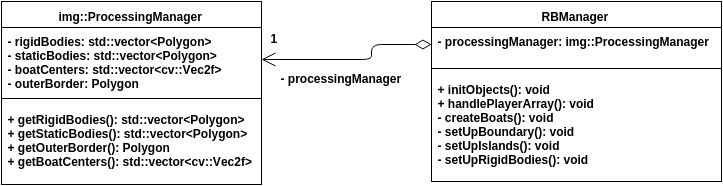
\includegraphics[scale=0.5]{img/RigidBodies/InterfaceRBImageRecogniton.png}
\caption{Interface between rigid bodies and image processing.}
\label{fig: interfaceRBIR}
\end{figure}


<<<<<<< HEAD
For each \texttt{Polygon} given from the \texttt{ProcessingManager}, we can calculate a center of mass. For rigid bodies (static or dynamic) we calculated the mean position of the polygon points as center of mass $\vec{x}$ and also the mean deviation $\hat{r}$ to approximate a radius $r$. To set up the boundary, we connect the polygon points one after another with the help of rectangular shaped rigid bodies. The mass and shape is assigned depending on the type of the body and its volume (mass=0: static body, mass$>$0: dynamic body). We end up with four different kinds of rigid bodies which we approximated as follows:
\begin{itemize}
\item \textbf{Boats:} \texttt{RBCircle} with position $\vec{x}$, radius $r=20$, mass$=0.6e4$ and moment of inertia$=1.2e7$.
\item \textbf{Islands:} \texttt{RBCircle} with position $\vec{x}$, radius $r=\hat{r}$, mass$=0$ and moment of inertia$=0$.
\item \textbf{Floating Objects:} \texttt{RBCircle} with position $\vec{x}$, radius $r=\hat{r}$, mass$=r^2$, and moment of inertia $=0$.
\item \textbf{Boundary:} Multiple \texttt{RBRectangle} connecting points of polygon, mass$=0$ and moment of inertia $=0$.
\end{itemize}
In the end, these new objects are added to the \texttt{btDiscreteDynamicWorld} and to the \texttt{RBCollection}.


As one can easily imagine there is a lot of freedom in the exact parameter choice; the values taken here were derived from playing the game and getting a user feedback.
%\begin{itemize}
%\item how to model boundaries
%\item how to create different rigid bodies
%\end{itemize}

\subsubsection{Interface to LBM}
\tododone[inline]{Benni}{Erik responsible for interface from RB \textbf{to LBM}}
\todointern[inline]{Erik}{Again, if someone feels like proofreading - but it's not very much.}
In order to get realistic interaction between the fluid field and the (among themselves interacting) rigid bodies, we decided to create an interface class \texttt{LBMRigidBodyObject}, in order to decouple the two parts of the program. The class was decided to:
\begin{itemize}
\item Wrap parts of the Rigid Body and Bullet functionality needed for the LBM simulation, such as calculating velocity on the outside of an object, or if a position was inside or outside the object. This would let the functionality be used int the LBM simulation without it having to implement Bullet, while also also isolating it from internal changes in the Rigid Body code.
\item Similarly, allow the LBM simulation to provide a force and torque from the fluid simulation on the rigid bodies for realistic interaction.
\item Also process some of the Rigid Body data to be used directly in the LBM simulation, such as delivering a list of LBM cells which were newly covered by the rigid body in the previous timestep. This was decided as the LBM simulation team was significantly smaller than the Rigid Body team, in order to balance the workload on the two groups.
\end{itemize}
In hindsight, this last point might not have been the most clever approach, as this processing was not yet in place when the LBM team wanted it, and since the raw data was not going to be needed if the processed data was there, the raw data was not provided by the interface In order to get their functionality, the LBM simulation then implemented Rigid Body-internal functionality, which caused several problem-causing dependencies that were painful to remove. A better approach might have been providing all possible needed raw functionality first, to allow the implementation at various points while still decoupling the two parts of the program. However, as all possible needs cannot always be foreseen when writing an interface, this approach might also not have been possible.

A summarizing UML diagram of the final interfacing can be found in \autoref{fig:LBMRigUML}.

\begin{figure}
	\includegraphics[width=\textwidth]{img/RigidBodies/RigidBodyLBM.png}
	\caption{Condensed UML diagram around the interface class \texttt{LBMRigidBodyObject}, which wraps and encapsulates functionality of Rigid Body and LBM classes.}
	\label{fig:LBMRigUML}
\end{figure}
%
%\begin{itemize}
%\item how to send important quantities (discretization of continuous RB into cells, velocity of RB...)
%\item how to receive important quantities (forces and torques from the fluid on the body)
%\end{itemize}

\subsubsection{Interface to Visualization}
\tododone[inline]{Benni}{Interface RB \textbf{to Visualization} done}
\todointern[inline]{Benni}{Erik or Friedrich please proofread}

For finally visualizing the rigid bodies we have to give access to the shape and the position of the rigid body. Our class \texttt{RBObject} already holds all this information. Therefore it was sufficient to grant -- through the \texttt{RBCollection} -- access to the \texttt{RBObject} objects:
\begin{itemize}
\item \texttt{getCenterOfMass()} and \texttt{getAngle()} give access to the position of the rigid body.
\item \texttt{getRBShape()} returns the \texttt{RBShape} of the body, which is either a \texttt{RBCircle} with its radius or a \texttt{RBRectangle} with the length of its two sides.
\end{itemize}
Representing shapes in an abstract way through the \texttt{RBShape} interface enabled us to completely hide Bullet from the visualization part of the pipeline while representing rigid body shapes in a proper and extensible way\footnote{Polygons could be easily added to our design, by simply adding a child class \texttt{RBPolygon} to the \texttt{RBShape} interface.}. 
